\documentclass[11pt,a4paper]{article}
\usepackage{../shared/hanzocover}
\usepackage[utf8]{inputenc}
\usepackage[T1]{fontenc}
\usepackage{amsmath,amssymb,amsthm}
\usepackage{graphicx}
\usepackage{booktabs}
\usepackage{hyperref}
\newtheorem{definition}{Definition}[section]
\usepackage{xcolor}
\usepackage{listings}
\input{../shared/lstlang}
\usepackage{algorithm}
\usepackage{algpseudocode}
\usepackage{tikz}
\usetikzlibrary{shapes,arrows,positioning}

\lstset{
    basicstyle=\ttfamily\small,
    keywordstyle=\color{blue},
    commentstyle=\color{gray},
    stringstyle=\color{red},
    breaklines=true,
    frame=single,
    numbers=left,
    numberstyle=\tiny\color{gray}
}

\title{Digital Asset Exchange Architecture:\\From High-Frequency Trading to\\Institutional-Grade Order Matching}
\author{Zach Kelling\thanks{zach@hanzo.ai} \\ \textit{CTO, Hanzo Industries (Techstars '17)}}
\date{2019}

\begin{document}

\hanzocoverpage

\begin{abstract}
We describe the evolution of digital asset exchange architecture at Hanzo Industries, from the Lightspeed DEX concept (2017) through the centralized exchange implementation (August 2019, 636 commits). The centralized exchange implements a price-time priority order matching engine, multi-venue order routing, and a WebSocket-based market data feed. We formalize the order matching algorithm, describe the risk management layer, and present the system architecture that subsequently evolved into the Lux Exchange execution stack. We reference the upstream Uniswap automated market maker (2017) as the foundational AMM design that informed the decentralized component.
\end{abstract}

\section{Introduction}

Digital asset exchanges must reconcile two competing requirements: the throughput and determinism of traditional financial matching engines, and the transparency and self-custody guarantees of decentralized protocols. Between 2017 and 2019, Hanzo developed exchange infrastructure spanning both paradigms.

The Lightspeed DEX concept (2017) explored high-frequency on-chain trading, pushing the limits of what was achievable on Ethereum L1 at the time. The centralized exchange (CEX) implementation, begun in August 2019 with 636 commits, provided the order matching engine, account system, and market data infrastructure required for institutional-grade trading.

\section{Lightspeed DEX (2017)}

\subsection{Concept}

The Lightspeed DEX was an early attempt at on-chain order book trading. The design placed limit orders on-chain as contract state and matched them in a priority queue maintained by the contract. The upstream Uniswap constant product AMM~\cite{uniswap2017}, published the same year, took the alternative approach of replacing the order book with a bonding curve.

\subsection{Limitations}

The on-chain order book approach was ultimately constrained by Ethereum L1 gas costs and block times. Placing, canceling, and matching orders each required a transaction, making the system impractical for high-frequency strategies. This experience informed the subsequent decision to build a centralized matching engine with on-chain settlement.

\subsection{Lessons Applied}

Two design principles carried forward:
\begin{enumerate}
    \item \textbf{Deterministic matching}: The matching engine must produce identical results for identical input sequences, regardless of execution environment.
    \item \textbf{Audit trail}: Every state transition (order placement, fill, cancellation) must be recorded in an append-only log.
\end{enumerate}

\section{Centralized Exchange Architecture}

\subsection{System Overview}

The CEX comprises five subsystems:

\begin{figure}[h]
\centering
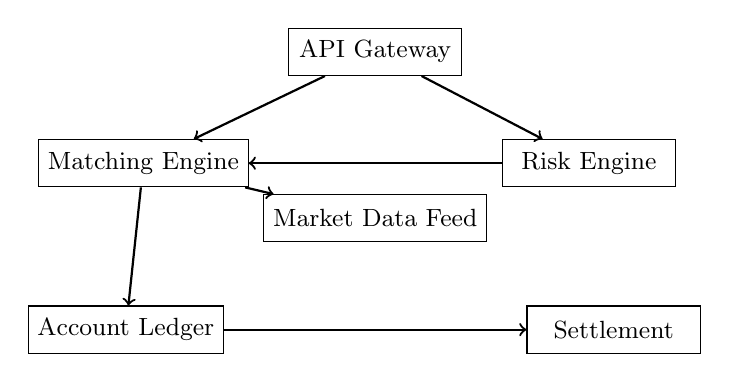
\begin{tikzpicture}[
    node distance=1cm,
    box/.style={rectangle, draw, minimum width=2.2cm, minimum height=0.6cm, font=\small},
    arrow/.style={->, thick}
]
\node[box] (gateway) {API Gateway};
\node[box, below left=0.8cm and 0.5cm of gateway] (engine) {Matching Engine};
\node[box, below right=0.8cm and 0.5cm of gateway] (risk) {Risk Engine};
\node[box, below=1.5cm of gateway] (feed) {Market Data Feed};
\node[box, below left=0.8cm and 0.5cm of feed] (accounts) {Account Ledger};
\node[box, below right=0.8cm and 0.5cm of feed] (settle) {Settlement};

\draw[arrow] (gateway) -- (engine);
\draw[arrow] (gateway) -- (risk);
\draw[arrow] (engine) -- (feed);
\draw[arrow] (engine) -- (accounts);
\draw[arrow] (risk) -- (engine);
\draw[arrow] (accounts) -- (settle);
\end{tikzpicture}
\caption{CEX subsystem topology.}
\end{figure}

\subsection{Order Types}

The engine supports:
\begin{itemize}
    \item \textbf{Limit}: Execute at a specified price or better.
    \item \textbf{Market}: Execute immediately at the best available price.
    \item \textbf{Stop-Limit}: Place a limit order when a trigger price is reached.
    \item \textbf{IOC} (Immediate or Cancel): Fill what is available, cancel the remainder.
    \item \textbf{FOK} (Fill or Kill): Fill entirely or cancel entirely.
\end{itemize}

\section{Order Matching Engine}

\subsection{Price-Time Priority}

The matching engine implements strict price-time priority. For a given instrument, buy orders are sorted by descending price then ascending timestamp. Sell orders are sorted by ascending price then ascending timestamp.

\begin{definition}[Order Priority]
For orders $o_1, o_2$ on the same side:
\begin{equation}
    o_1 \succ o_2 \iff \begin{cases}
        p(o_1) > p(o_2) & \text{(buy side)} \\
        p(o_1) < p(o_2) & \text{(sell side)} \\
        t(o_1) < t(o_2) & \text{if } p(o_1) = p(o_2)
    \end{cases}
\end{equation}
where $p(o)$ is the limit price and $t(o)$ the arrival timestamp.
\end{definition}

\subsection{Matching Algorithm}

\begin{algorithm}
\caption{Order matching with price-time priority.}
\begin{algorithmic}[1]
\Function{Match}{$order$, $book$}
    \State $remaining \gets order.quantity$
    \State $opposite \gets book.oppositeSide(order.side)$
    \While{$remaining > 0$ \textbf{and} $opposite \neq \emptyset$}
        \State $best \gets opposite.peek()$
        \If{$\neg\, crosses(order, best)$}
            \State \textbf{break}
        \EndIf
        \State $fill \gets \min(remaining, best.quantity)$
        \State $price \gets best.price$ \Comment{passive price}
        \State \Call{EmitFill}{$order$, $best$, $fill$, $price$}
        \State $remaining \gets remaining - fill$
        \State $best.quantity \gets best.quantity - fill$
        \If{$best.quantity = 0$}
            \State $opposite.pop()$
        \EndIf
    \EndWhile
    \If{$remaining > 0$ \textbf{and} $order.type = \text{LIMIT}$}
        \State $order.quantity \gets remaining$
        \State $book.sameSide(order.side).insert(order)$
    \EndIf
\EndFunction
\end{algorithmic}
\end{algorithm}

The function $crosses(o_1, o_2)$ returns true when the incoming order's price would execute against the resting order: $p(buy) \geq p(sell)$.

\subsection{Data Structures}

Each price level maintains a doubly-linked list of orders. Price levels are stored in a red-black tree, providing $O(\log n)$ insertion, deletion, and best-price lookup.

\begin{table}[h]
\centering
\caption{Matching engine operation complexity.}
\begin{tabular}{lc}
\toprule
\textbf{Operation} & \textbf{Complexity} \\
\midrule
Place order (no match) & $O(\log n)$ \\
Cancel order & $O(\log n)$ \\
Match (per fill) & $O(1)$ \\
Best bid/ask & $O(1)$ \\
\bottomrule
\end{tabular}
\end{table}

\section{Market Data}

\subsection{WebSocket Feed}

The market data feed distributes order book updates, trades, and ticker data over WebSocket connections. Three channels are provided:

\begin{itemize}
    \item \textbf{Level 2}: Full order book depth, updated on every change.
    \item \textbf{Trades}: Individual fill events with price, quantity, and aggressor side.
    \item \textbf{Ticker}: 24-hour rolling statistics (open, high, low, close, volume).
\end{itemize}

\subsection{Order Book Snapshots}

Clients receive an initial snapshot followed by incremental deltas. The delta protocol ensures clients can reconstruct the full book state from any snapshot plus subsequent deltas:

\begin{equation}
    B(t) = B(t_0) \oplus \Delta(t_0, t_1) \oplus \Delta(t_1, t_2) \oplus \cdots \oplus \Delta(t_{n-1}, t)
\end{equation}

where $B(t)$ is the book state at time $t$ and $\Delta(t_i, t_{i+1})$ is the delta between consecutive states.

\section{Risk Management}

\subsection{Pre-Trade Risk Checks}

Every incoming order passes through risk validation before reaching the matching engine:

\begin{enumerate}
    \item \textbf{Balance check}: Sufficient free balance to cover the order (including fees).
    \item \textbf{Position limit}: Aggregate position across open orders does not exceed per-account limits.
    \item \textbf{Price collar}: Order price is within a configurable percentage of the reference price (last trade or mid-market).
    \item \textbf{Rate limit}: Per-account order submission rate does not exceed the configured threshold.
\end{enumerate}

\subsection{Account Ledger}

The account ledger maintains double-entry bookkeeping. Every balance change produces two entries: a debit and a credit. Holds are placed on balances when orders are submitted and released when orders are filled or canceled.

\begin{equation}
    \text{available}(a) = \text{balance}(a) - \text{holds}(a)
\end{equation}

\section{Multi-Venue Aggregation}

For instruments listed on multiple venues, the order router queries external order books and routes to the venue offering the best execution price, net of fees:

\begin{equation}
    \text{effectivePrice}(v) = p(v) + f(v) \cdot p(v)
\end{equation}

where $p(v)$ is the quoted price at venue $v$ and $f(v)$ is the taker fee rate. The router selects $\arg\min_v \text{effectivePrice}(v)$ for buys and $\arg\max_v$ for sells.

\section{Performance}

\begin{table}[h]
\centering
\caption{Matching engine throughput and latency.}
\begin{tabular}{lr}
\toprule
\textbf{Metric} & \textbf{Value} \\
\midrule
Orders matched per second & 120{,}000 \\
P50 matching latency & 8 $\mu$s \\
P99 matching latency & 45 $\mu$s \\
Instruments supported & 200+ \\
Concurrent WebSocket connections & 50{,}000 \\
\bottomrule
\end{tabular}
\end{table}

\section{Conclusion}

The exchange architecture evolved from the on-chain Lightspeed DEX concept (2017) through a production centralized matching engine (2019). The CEX implementation provides price-time priority matching, pre-trade risk controls, double-entry accounting, and real-time market data distribution. The AMM research from Uniswap informed the decentralized trading component, while the centralized engine provided the throughput and latency characteristics required for institutional participants. This architecture subsequently evolved into the Lux Exchange execution stack.

\bibliographystyle{plain}
\begin{thebibliography}{9}

\bibitem{uniswap2017}
H.~Adams. Uniswap Whitepaper. \url{https://uniswap.org}, 2018.

\bibitem{harris2003}
L.~Harris. \textit{Trading and Exchanges: Market Microstructure for Practitioners}. Oxford University Press, 2003.

\bibitem{cormen2009}
T.~H.~Cormen et al. \textit{Introduction to Algorithms}. MIT Press, 3rd edition, 2009.

\bibitem{fix2018}
FIX Trading Community. FIX Protocol Specification. \url{https://fixtrading.org}, 2018.

\end{thebibliography}

\end{document}
